\documentclass{beamer}
%[aspectratio=169]   \usepackage[czech]{babel}
\usepackage{apo-lecture}
\usepackage{pdfpages}
\usepackage{pdfcomment}
\usepackage{listings}
\usepackage{array,multirow}

\subtitle{Lekce 10. Překlad jazyka C}
\author{Pavel Píša \phantom{xxxxxxxxx} Petr Štěpán \\ \small\texttt{pisa@fel.cvut.cz}\phantom{xxxx}\small\texttt{stepan@fel.cvut.cz}}
\begin{document}

\maketitle

\section{Volání funkce}

\begin{frame}
\frametitle{Cíl dnešní přednášky}

\begin{itemize}
 \item Zjistit, jak se program v jazyce C přeloží na strojové instrukce například procesoru RISC-V
\end{itemize}
\end{frame}


\begin{frame}
\frametitle{Jak se překládá program v C}

Jednoduchý příklad: překlad \texttt{a = b + c;}
\begin{enumerate}
 \item Přiřadit proměnným registry, např. b - t0, c - t1, a - t0
 \item Nahrát do registrů hodnoty proměnných: 
 
 \texttt{lw t0, \&b(gp)}; 
 
 \texttt{lw t1, \&c(gp)}
 \item Provést výpočet: 
 
 \texttt{add t0, t0, t1}
 \item Uložit hodnotu do proměnné \texttt{a}: 
 
 \texttt{sw t0, \&a(gp)} 
\end{enumerate}

\bigskip

\begin{itemize}
 \item Obecné výrazy se analyzují pomocí bezkontextových gramatik - definuje všechny výrazy možné v jazyce C.
 \item Výše uvedený překlad je bez optimalizace, uloží hodnotu do proměnné a, v dalším kroku ji může opět nahrávat z paměti třeba i do stejného registru. 
 \item Pokud by adresy proměnných nebyly dosažitelné registrem \texttt{gp}, je nutné před instrukcí \texttt{lw} nahrát adresu proměnné.
\end{itemize}

\end{frame}


\begin{frame}[fragile]
\frametitle{Překlad konstrukce while}

Složitější překlad: překlad konstrukce \texttt{while (cond) body;}
\begin{columns}
\begin{column}{0.7\textwidth}
\small
\begin{itemize}
 \item analýza bezkontextové gramatiky jazyka detekuje while kontrukci
 \item rekurzivně se zajistí překlad podmínky \texttt{cond} na množinu instrukcí \texttt{COND} a překlad těla cyklu \texttt{body} na množinu instrukcí \texttt{BODY}.
 \item vygeneruje se instrukce \texttt{j cond\_1}, skok na něstí cond\_1
 \item vloží se návěstí \texttt{body\_1}
 \item vloží se všechny instrukce těla cyklu \texttt{BODY}
 \item vloží se návěstí \texttt{cond\_1}
 \item vloží se instrukce pro generování podmínky \texttt{COND}, výsledek bude např. v registru t0
 \item vygeneruje se instrukce \texttt{bne t0, zero, body\_1}
\end{itemize}
\end{column}
\begin{column}{0.3\textwidth}  
\begin{minted}[fontsize=\footnotesize]{gas}
  j  cond_1
    
body_1:

  BODY

cond_1:

  COND
    
  bne t0, zero, body_1
\end{minted}
\end{column}
\end{columns}

\end{frame}


\begin{frame}
\frametitle{Jak se přeložit funkci?}

Pro překlad funkce např. \texttt{int secti(int a, int b);} je nutné vymyslet:
\begin{itemize}
 \item Jak předat parametry a,b?
 \item Jak předat výsledek secti?
 \item Jakou instrukci dát na konec funkce, kam skočit?
\end{itemize}

Volající (caller) a volaný (callee) se musí dohodnout na těchto otázkách, aby si rozuměli.
\begin{itemize}
 \item Překlad volaného může být na jiném počítači, jiným překladačem (typicky knihovny) než překlad volajícího - Vaším překladačem na Vašem počítači.
 \item Je nutné definovat konvenci, typ konvence volání funkce musí být v hlavičce objektových souborů (a tím i knohoven) aby zajistila správnost předání dat a získání návratové hodnoty.
\end{itemize}
\end{frame}



\begin{frame}[fragile]
\frametitle{Konvence volání funkce pro RISC-V}

\begin{itemize}
 \item Parametry funkce uloží volající do registrů a0, ... , a7
\begin{itemize}
 \item Co když bude parametrů více? Probereme v této přednášce později.
\end{itemize}
 \item Výsledek funkce bude v registrech a0 a a1.
\begin{itemize}
 \item Co když se výsledek nevejde do těchto dvou registrů?
 \item Volající musí připravit místo, kam se výsledek uloží.
 \item Ukazatel na adresu výsledku předá jako skrytý parametr do funkce.
 \item Volaný uloží výsledek funkce rovnou na připravenou adresu.
 \item Podívejte se na příklad ret\_struct.c.
\end{itemize}
\end{itemize}

\begin{columns}
\begin{column}{0.45\textwidth}  
\begin{minted}[fontsize=\footnotesize]{c}
struct a {
  int a, b, c, d;
};

struct a permut(int x, int y);

struct a t;

t = permut(1, 2, 3, 4);
\end{minted}
\end{column}
\begin{column}{0.55\textwidth}  
\begin{minted}[fontsize=\footnotesize]{c}
struct a {
  int a, b, c, d;
};

void permut(struct a *r, int x, int y);

struct a t;

permut(&t, 1, 2, 3, 4);
\end{minted}
\end{column}
\end{columns}
\end{frame}


\begin{frame}[fragile]
\frametitle{Jak přeložit návrat z funkce?}

\begin{columns}
\begin{column}{0.3\textwidth}  
\begin{minted}[fontsize=\footnotesize]{gas}
[0x100]  j  soucet
         
         ...
         
[0x254]  j  soucet
    

soucet:

    ...
    
    j ? 
0x104 nebo 0x258?
nebo jinam
\end{minted}
\end{column}
\begin{column}{0.7\textwidth}
\begin{itemize}
 \item funkce soucet může být volána z mnoha různých míst programu
 \item nelze vygenerovat adresu skoku návrat z funkce v době překladu
 \item návratová hodnota musí být nastavena volajícím
 \item konvence volání funkce -- návratová hodnota adresy je uložena v registru ra (return address) -- registr x1
 \item potřebujeme instrukci, která skočí na adresu uloženou v registru
 \item hodila by se i instrukce, která uloží do registru ra adresu následující instrukce
\end{itemize}
\end{column}
\end{columns}
\end{frame}



\begin{frame}
\frametitle{Instrukce jal, jalr (ret, jr)}

Instrukce jal "rd," address
\begin{itemize}
 \item skoč na adresu address (21 bitů, nejnižší bit defaultně 0) a do registru rd ulož hodnotu PC+4
 \item pokud neuvedete registr rd, tak se standardně doplní x1
 \item pokud chceme jen skok (instrukce j), tak se PC+4 uloží do registru x0
\end{itemize}

Instrukce jalr rd, rs1, imm12
\begin{itemize}
 \item skoč na adresu rs1 + imm12 a do registru rd ulož hodnotu PC+4
 \item pokud neuvedete registr rd, tak se standardně doplní x1
 \item pokud chceme jen návrat z funkce, lze použít pro rd registr x0
\end{itemize}
\end{frame}


\begin{frame}
\frametitle{Implemetace jal a jalr}

\begin{center}

\includegraphics[width=0.8\textwidth]{Qtrvsim-jalr.pdf}
\end{center}

Kvíz: Kolik různých čar byste uměli vysvětlit A žádnou, B asi třetinu, C asi polovinu, D téměř všechny.
\end{frame}


\begin{frame}
\frametitle{Simulace Jalr}

\begin{center}

\includegraphics[width=0.8\textwidth]{Jalr-exec.pdf}
\end{center}

\end{frame}



\begin{frame}
\frametitle{Řídicí hazard při Implemetaci jalr}

\begin{center}

\includegraphics[width=0.8\textwidth]{Jalr-mem.pdf}
\end{center}

\end{frame}



\begin{frame}
\frametitle{Co když funkce ve svém těle volá jinou funkci?}

Volající připraví argumenty do registrů a0 až a7 a do registru ra návratovou hodnotu.

\bigskip

Jak ale vyřešit, když funkce ve svém těle volá jinou funkci?

\bigskip

Je nutné někam uložit registr ra, registry a0-a7, ale kam?


\begin{itemize}
 \item Pro uložení dočasných proměnných slouží: Activation record nebo také activation frame. 
 \item Tento záznam, nebo rámec se uloží na zásobník (anglicky call stack nebo stack frame).
\end{itemize}
\end{frame}


\begin{frame}
\frametitle{Zásobník}

\begin{columns}
\begin{column}{0.7\textwidth}
Zásobník je datová struktura LIFO (Last In First Out) -- neboli poslední vložená data jdou první ven
\begin{itemize}
 \item push -- vlož data do zásobníku
 \item pop -- vyber data ze zásobníku
\end{itemize}

Implemetace zásobníku registrem sp (x2):
\begin{itemize}
 \item push 
 
\texttt{addi sp, sp, -4 \phantom{xx}}  -- alokace místa

\texttt{sw \phantom{xx}x10, 0(sp) \phantom{xx}}  -- uložení hodnoty
 
 \item pop

\texttt{lw \phantom{xx}x10, 0(sp) \phantom{xx}}  -- načtení hodnoty

\texttt{addi sp, sp, 4 \phantom{xxx}}  -- dealokace místa

\end{itemize}

\end{column}
\hfill
\begin{column}{0.3\textwidth}  
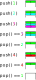
\includegraphics[width=0.9\textwidth]{zasobnik.pdf}
\end{column}
\end{columns}

\end{frame}

\begin{frame}
\frametitle{Co se ukládá na zásobník?}

Activation frame obsahuje:
\begin{itemize}
 \item Parametry funkce a návratová adresa, pokud se v těle funkce volá jiná funkce.
 \item Lokální proměnné funkce, které eistují jen v průběhu vykonávání funkce.
 \item Podle konvence překladu funkce se nesmí po návratu z funkce změnit hodnota registrů s0-s11
\begin{itemize}
 \item Registr s0 se někdy používá jako ukazatel na Activation frame a nazývá se fp -- frame pointer
 \item Registr fp se využívá jako pevný ukazatel na předem dané místo rámce a tím ho lze použít k odkazu na lokální proměnné funkce a parametry funkcí.
\end{itemize}
\end{itemize}
\end{frame}


\begin{frame}
\frametitle{Konvence volání funkce}

Každý regiter buď nastavuje a je za něj zodpovědný volající (caller), nebo volaný (callee). 

\begin{tabular}{|c|c|p{4cm}|c|}\hline
Symbolické & Registr & Popis & Ukládá \\
   jméno   &         &       &        \\ \hline
a0 - a7 & x10 - x17 & vstupní parametry funkce & volající \\\hline
a0, a1 & x10, x11 & výstupní hodnota funkce & volající \\\hline
ra & x1 & návratová adresa & volající \\\hline
t0 - t6 & x5-7, x28-x31 & dočasné registry & volající\\\hline
s0 - s11 & x8-9, x18-x27 & ukládané registry & volaný\\\hline
sp & x2 & ukazatel zásobníku & volaný\\\hline
gp & x3 & globální ukazatel & -- --\\\hline
tp & x4 & ukazatel na vlákno (thread) & -- --\\\hline
\end{tabular}
\end{frame}


\begin{frame}
\frametitle{Konvence volání funkce 32 bitového systému}

\begin{itemize}
 \item char, short, int, long, float, pointer -- každý parametr jeden registr
 \item long long int, double -- každý parametr dva registry
 \item struct předávaná hodnotou se kopíruje do tolika registrů, kolik je potřeba
 \item pokud je překládáno pro RISC-V s rozšířením pro práci s reálnými čísly, pak se pro předávání float, double i struktur využijí registry f10 -- f17 označovaných také fa0 -- fa7
 \item pokud se parametry nevejdou do registrů a0-a7, tak se přebývající parametry umístí na zásobník do rámce nově volané funkce
\end{itemize}
\end{frame}


\begin{frame}[fragile]
\frametitle{Volání funkce}

\begin{columns}
\begin{column}{0.5\textwidth}
Volání funkce s maximálně 8 parametry:

\begin{minted}[fontsize=\footnotesize]{c}
t = secti(1, 2, 3, 4);
\end{minted}

Překlad do RISC-V
\begin{minted}[fontsize=\footnotesize]{gas}
li  a3,4
li  a2,3
li  a1,2
li  a0,1
jal ra,10054 <secti>
\end{minted}

\end{column}
\begin{column}{0.5\textwidth}  
Volání funkce s 10 parametry:

\begin{minted}[fontsize=\footnotesize]{c}
t = secti(1, 2, 3, 4, 5, 
          6, 7, 8, 9, 10);
\end{minted}

Překlad do RISC-V
\begin{minted}[fontsize=\footnotesize]{gas}
li  a5,10
sw  a5,4(sp)
li  a5,9
sw  a5,0(sp)
li  a7,8
li  a6,7
li  a5,6
li  a4,5
li  a3,4
li  a2,3
li  a1,2
li  a0,1
jal ra,10054 <secti>
\end{minted}
\end{column}
\end{columns}


\end{frame}



\begin{frame}
\frametitle{Překlad funkce - jednoduchá funkce}

Příklad s málo parametry bez vnitřního volání funkce se čtyřmi lokálními proměnými.
\begin{columns}
\begin{column}{0.65\textwidth}
\begin{itemize}
 \item Alokace místa pro lokální proměnné 
 
 \texttt{addi  sp,sp,-16}
 \item Lokální proměnné na adresách: 
 
 0(sp), 4(sp), 8(sp), 12(sp)
\begin{itemize}
 \item Pokud to lze, jsou proměnné umístěny v registrech a stack by se vůbec nepoužil
\end{itemize}
\end{itemize}

Ukončení funkce:
\begin{itemize}
 \item Dealokace místa pro lokální proměnné 
 
 \texttt{addi  sp,sp,16}
 \item Návrat z funkce 
 
 \texttt{jalr 0(x1)} -- \texttt{ret} 
\end{itemize}
\end{column}
\begin{column}{0.35\textwidth}  
\includegraphics[width=0.9\textwidth]{jednoducha_fce.pdf}
\end{column}
\end{columns}

\end{frame}


\begin{frame}[fragile,shrink=5]
\frametitle{Překlad funkce}

Příklad s 10 parametry, volání funkce uvnitř funkce, se dvěma lokálními proměnými.

\begin{columns}
\begin{column}{0.32\textwidth}
Začátek funkce:

\begin{minted}[fontsize=\footnotesize]{gas}
addi  sp,sp,-48
sw  ra,44(sp)
sw  s0,40(sp)
sw  s1,36(sp)
sw  s2,32(sp)
sw  s3,28(sp)
sw  s4,24(sp)
\end{minted}
\end{column}   
\begin{column}{0.32\textwidth}
Ukončení funkce:

\begin{minted}[fontsize=\footnotesize]{gas}
lw   ra,44(sp)
lw   s0,40(sp)
lw   s1,36(sp)
lw   s2,32(sp)
lw   s3,28(sp)
lw   s4,24(sp)
addi sp,sp,48
ret
\end{minted}
\end{column}
\begin{column}{0.35\textwidth}  
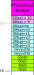
\includegraphics[width=0.7\textwidth]{slozita_fce.pdf}
\end{column}
\end{columns}
\end{frame}



\begin{frame}[shrink=5]
\frametitle{Ukazatel na rámec funkce}

\begin{itemize}
 \item Ukazatel na rámec funkce udržuje v RISC-V hodnotu sp při vstupu do funkce
 \item Pro fp (frame pointer) je využit registr s0, je to tedy registr, který musí volaný uložit a při návratu z funkce obnovit
 \item Výhody použití fp
\begin{itemize}
 \item Pevně nastavené ukazatele na argumenty a lokální proměnné funkce, pokud se sp v těle mění (např. argumenty pro volné funkce), pak se mění i posunutí vshledem k sp pro přístup k argumentům a lokálním funkcím.
 \item Přehldnější zásobník pro debugery a při tzv. odvinutí zásobníku.
\begin{itemize}
 \item Odvinutí zásobníku se provádí v C++ při výskytu výjimky ve funkci, kdy je ale výjimka zpracována až ve funkci nadřazené, která tuto funkci volala.
 \item Pro zpracování výjimky je nutné nastavit zásobník do stavu, ve které nadřazená funkce volala funkci, ve které výjimka nastala.
\end{itemize}
\end{itemize}
 \item Nevýhody použití fp:
\begin{itemize}
 \item Zpomaluje program, jedná se sice jen o několik instrukcí při vstupu a ukončení funkce, ale pokud se funkce volá často a její tělo je krátké, může to být i značné zpomalení.
 \item Fp obsadí registr s0, který by se dal využít pro uchování hodnoty. Pokud by došli volné registry, pak se hodnota musí uložit na zásobník do paměti RAM (přes cache) což je pomalejší než využití registru.
\end{itemize}
\end{itemize}
\end{frame}


\begin{frame}[fragile,shrink=5]
\frametitle{Překlad funkce s ukazatelem na rámec funkce}

Pro překlad gcc pro RISC-V je nutné využít přepínač \texttt{-fno-omit-frame-pointer}
\begin{columns}
\begin{column}{0.32\textwidth}
Začátek funkce:

\begin{minted}[fontsize=\footnotesize]{gas}
addi sp,sp,-48
sw   ra,44(sp)
sw   s0,40(sp)
sw   s1,36(sp)
sw   s2,32(sp)
sw   s3,28(sp)
sw   s4,24(sp)
sw   s5,20(sp)
addi s0,sp,48
\end{minted}
\end{column}   
\begin{column}{0.32\textwidth}
Odkaz na lokální proměnnou:

\begin{minted}[fontsize=\footnotesize]{gas}
sw	a0,-36(s0)  # sw a0, 12(sp)
\end{minted}


Ukončení funkce:

\begin{minted}[fontsize=\footnotesize]{gas}
lw   ra,44(sp)
lw   s0,40(sp)
lw   s1,36(sp)
lw   s2,32(sp)
lw   s3,28(sp)
lw   s4,24(sp)
lw   s5,20(sp)
addi sp,sp,48
ret
\end{minted}
\end{column}
\begin{column}{0.35\textwidth}  
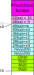
\includegraphics[width=0.7\textwidth]{slozita_fce_fp.pdf}
\end{column}
\end{columns}
\end{frame}



\begin{frame}
\frametitle{Rozložení běžícího programu v paměti}

Obrázek 

\begin{itemize}
 \item Popis 
 \item Zachování hodnot vybraných registrů
 \item Lokální proměnné funkce
 \item Návratová hodnota funkce
\end{itemize}
\end{frame}


\begin{frame}
\frametitle{Jak se pracuje s char a short?}

ukázky překladu.

\end{frame}


\begin{frame}
\frametitle{Útok na program přes zásobník}

obrázek s použitím pole ke změně návratové hodnoty

OSY

\end{frame}



\begin{frame}[fragile]
\frametitle{Proměnný počet parametrů va\_list}

Definice funkce s proměnným počtem parametrů:

\begin{columns}
\begin{column}{0.4\textwidth}
\begin{minted}[fontsize=\footnotesize]{c}
#include <stdarg.h>

int secti(int n, ...) {
  int souc = 0;
  int i;
  va_list ap;
  
  va_start(ap, n);
  for (i=0; i<n; i++) {
    souc+=va_arg(ap,int);
  }
  va_end(ap);
  return souc;
}
\end{minted}
\end{column}   
\begin{column}{0.6\textwidth}
Volání funkce:

\begin{minted}[fontsize=\footnotesize]{c}
int  main() {
  printf("Soucet %d\n", secti(10, 1,2,3,
                         4,5,6,7,8,9,10);
  printf("Soucet %d\n", secti(2, 1,2);
  printf("Soucet %d\n", secti(8, 1,2,3,
                              4,5,6,7,8);
}
\end{minted}
\end{column}
\end{columns}

\end{frame}

\begin{frame}
\frametitle{Proměnný počet parametrů va\_list}

Překlad

\end{frame}


\section {Systémová volání}

\begin{frame}
\frametitle{Ochrana OS}


\end{frame}

\begin{frame}
\frametitle{Ochrana OS}


\end{frame}


\end{document}

